\section{Phương pháp đề xuất}

\subsection{Mô hình}
Sau khi chạy thực nghiệm và đánh giá các phương pháp gợi ý trên dữ liệu MOOCCubeX \cite{mooccubex}, nhóm đã chọn ra được phương pháp tốt nhất là KGAT model (chi tiết kết quả trong mục 5). Vì vậy trong phần này, nhóm sẽ trình bày cách chuyển đổi từ input sang output của mô hình KGAT, còn phương pháp chuẩn bị dữ liệu sẽ được trình bày ở phần 5.

\begin{figure}[h]
    \centering
    % Placeholder for Image 1
    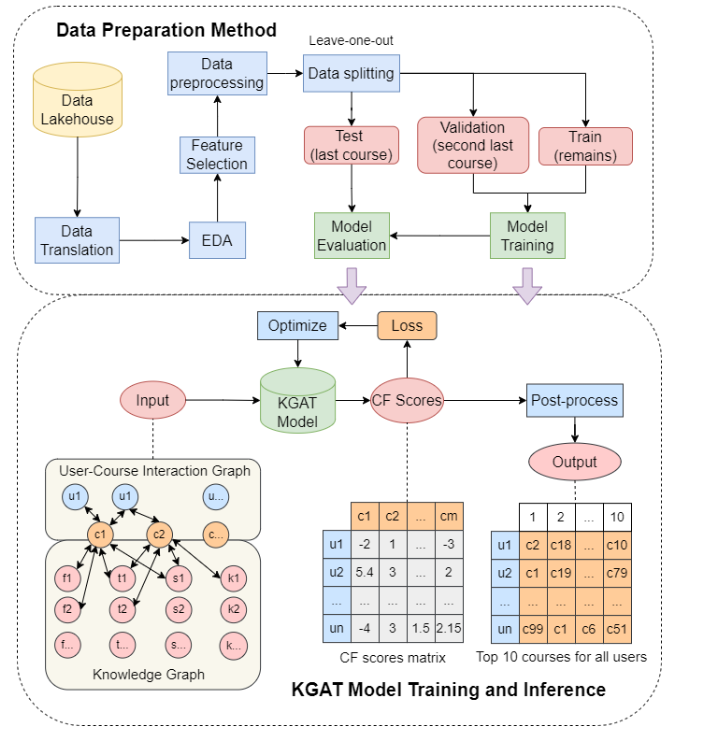
\includegraphics[width=0.8\textwidth]{figures/69.png}
    \caption{Hình minh họa quy trình thực nghiệm bài toán với cách tiếp cận sử dụng mô hình KGAT}
    \label{fig:image1}
\end{figure}

Input của mô hình là collaborative knowledge graph chứa 2 đồ thị thành phần như Hình~\ref{fig:image1}: user-item bipartite graph và knowledge graph. User-item bipartite graph biểu diễn mối quan hệ người dùng đã đăng ký khóa học nào và mối quan hệ ngược lại, nghĩa là khóa học được đăng ký bởi user nào. Còn knowledge graph biểu diễn mỗi quan hệ giữa khóa học và các thuộc tính của nó. Nếu xét node xuất phát là khóa học, đồ thị này sẽ có 4 loại quan hệ: khóa học có khái niệm (concept) nào; khóa học thuộc lĩnh vực (field) nào; khóa học được dạy bởi giáo viên (teacher) nào; khóa học được tổ chức bởi trường (school) nào. Và tính thêm chiều ngược lại, ta sẽ có tổng cộng $4 \times 2 = 8$ loại quan hệ giữa khóa học và các thuộc tính.

Khi nhận được input, model sẽ trả về một ma trận collaborative scores $\text{cf\_scores} \in \mathbb{R}^{n_{\text{users}} \times n_{\text{courses}}}$, với mỗi phần tử $\text{cf\_scores}_{i,j} \in \mathbb{R}$ $(i,j \in \mathbb{N}; 0 \leq i < n_{\text{users}}; 0 \leq j < n_{\text{courses}})$ cho biết mức độ phù hợp giữa $\text{user}_i$ và $\text{course}_j$. Nếu giá trị này càng lớn thì $\text{user}_i$ càng phù hợp với $\text{course}_j$ và ngược lại.

Sau đó, giai đoạn hậu xử lý (Hình~\ref{fig:image2}) sẽ gán giá trị âm vô cùng cho $\text{cf\_scores}[i, j]$ nếu $\text{user}_i$ đã đăng ký $\text{course}_j$; tiếp đến argsort giảm dần theo chiều $\text{axis} = 1$ (để các khóa học mà $\text{user}_i$ đã đăng ký không bị đề xuất lại) rồi lấy top 10 khóa học có score cao nhất ứng với mỗi user để làm output.

\begin{figure}[h]
    \centering
    % Placeholder for Image 2
    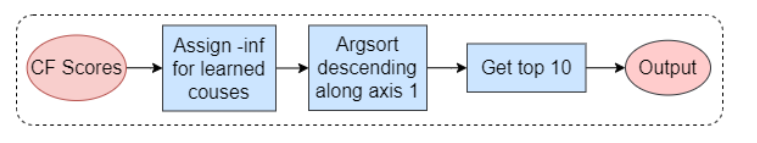
\includegraphics[width=0.8\textwidth]{figures/70.png}
    \caption{Hình minh họa giai đoạn hậu xử lý để lọc ra được top-k khóa học được đề xuất}
    \label{fig:image2}
\end{figure}

